\documentclass{article}
\usepackage{eecstex}
\usepackage{pgfplots}

\title{Homework 1}
\author{Bryan Ngo}
\date{2022-01-19}

\begin{document}

\maketitle

\setcounter{section}{1}

\section{}

\subsection{}

\begin{theorem}
    The system \(L\) is not time invariant.
\end{theorem}
\begin{proof}
    We can represent a time-delayed signal as a linear combination of the other 3 signals.
    We can represent the 3 input signals in a matrix
    \begin{equation}
        \bm{X} =
        \begin{bmatrix}
           -2 & -2 & 0 \\
           1 & 1 & 1 \\
           -2 & 0 & 1 
        \end{bmatrix}
    \end{equation}
    Then, we can find the linear combination necessary to create a time delayed signal (for example, \(x_2[n - 1]\)) by solving the system of equations
    \begin{equation}
        \bm{Xa} =
        \begin{bmatrix}
            0 \\
            -2 \\
            1
        \end{bmatrix}
    \end{equation}
    where we get \(\bm{a} = \begin{bmatrix}
        -\frac{3}{2} & \frac{3}{2} & -2
    \end{bmatrix}^\top\).
    Thus, we have
    \begin{equation}
        x_2[n - 1] = -\frac{3}{2} x_1[n] + \frac{3}{2} x_2[n] - 2x_3[n]
    \end{equation}
    Calculating \(-\frac{3}{2} y_1[n] + \frac{3}{2} y_2[n] - 2y_3[n]\),
    we get the following plot:
    \begin{center}
        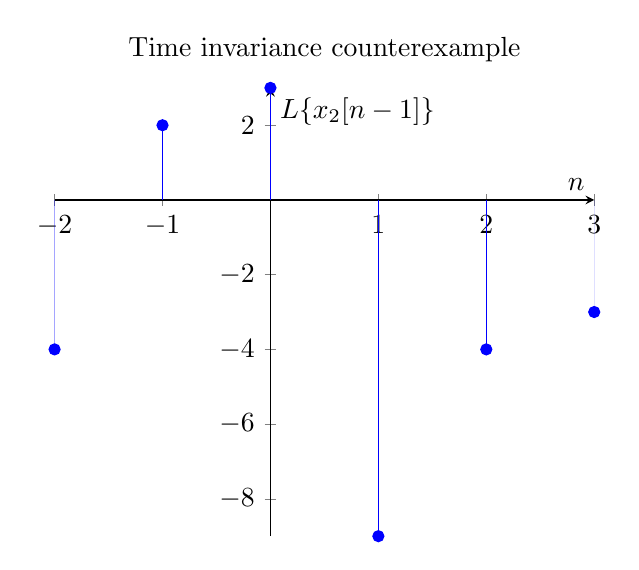
\begin{tikzpicture}
            \begin{axis}[
                xlabel=\(n\), ylabel={\(L\{x_2[n - 1]\}\)},
                title={Time invariance counterexample},
                axis lines=middle
            ]
            \addplot[
                ycomb,
                color=blue,
                mark=*
            ]
            coordinates {
                (-2, -4)
                (-1, 2)
                (0, 3)
                (1, -9)
                (2, -4)
                (3, -3)
            };
            \end{axis}
        \end{tikzpicture}
        \begin{tikzpicture}
            \begin{axis}[
                xlabel=\(n\), ylabel={\(y_2[n - 1]\)},
                title={Expected output signal},
                axis lines=middle
            ]
            \addplot[
                ycomb,
                color=blue,
                mark=*
            ]
            coordinates {
                (0, -1)
                (1, 1)
                (2, -3)
                (3, -0)
                (4, -1)
            };
            \end{axis}
        \end{tikzpicture}
    \end{center}
\end{proof}

\subsection{}

We can represent the delta function as
\begin{equation}
    \delta[n] = \frac{1}{2} (x_1[n] - x_2[n] + 2x_3[n])
\end{equation}
Using the properties of linear systems, we can find the impulse response
\begin{equation}
    h[n] = \frac{1}{2} (y_1[n] - y_2[n] + 2y_3[n])
\end{equation}
which gives us the following plot:
\begin{center}
    \begin{tikzpicture}
        \begin{axis}[
            xlabel=\(n\), ylabel={\(L\{\delta[n]\}\)},
            title={Impulse response},
            axis lines=middle
        ]
        \addplot[
            ycomb,
            color=blue,
            mark=*
        ]
        coordinates {
            (-2, 2)
            (-1, 1)
            (0, -2)
            (1, 3)
            (2, 2)
            (3, 1)
        };
        \end{axis}
    \end{tikzpicture}
\end{center}

\section{}

\begin{align}
    y[n] - ay[n - 1] &= x[n] \\
    y[0] &= 1
\end{align}

\subsection{}

For the homogenuous solution, assume that \(y_h[n] = A\lambda^n\).
Then,
\begin{align}
    A\lambda^n - aA\lambda^{n - 1} &= 0 \\
    1 - a\lambda^{-1} &= 0 \\
    \implies \lambda &= a
    \implies y_h[n] = Aa^n
\end{align}
Finding the particular solution,
\begin{equation}
    \begin{array}[]{||c|c||}
        \hline
        n & y_p[n] \\
        \hline
        0 & 1 \\
        N & f[N] = \alpha f[0] = \alpha \\
        2N & f[2N] = \alpha f[N] = \alpha^2 \\
        \vdots & \vdots \\
        \hline
    \end{array}
\end{equation}

\end{document}
